\begin{lecture}{H}{Database Administration}

\begin{slide}
\Heading{Database Administration}
Database installations are typically ...
\begin{itemize}
\vspace{-1ex}\item used by {\em{many}} casual users ~ {\small (typically via a web interface)}
\vspace{-1ex}\item used by {\em{few}} developers ~ {\small (who build schemas and applications)}
\vspace{-1ex}\item managed by {\em{one}} DB administrator ~ {\small (or a small team of DBAs)}
\end{itemize}
\vspace*{1cm}\begin{center}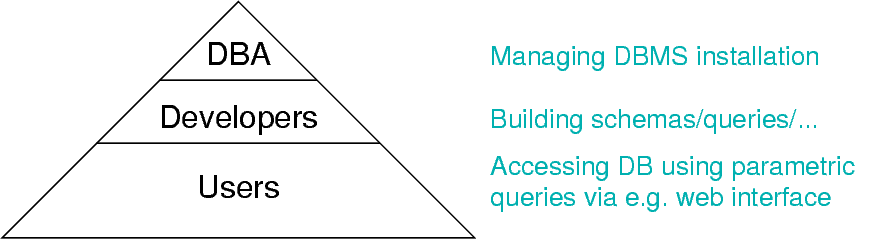
\psfig{file=Pic/usage.ps}\end{center}
\end{slide}

\begin{slide}
\ContHeading{Database Administration}
Tasks of the database administrator:
\begin{itemize}
\item manage the database installation \\
	{\small (including configuring system parameters, running the server, back-ups, ...)}
\item create users and specify what they can/cannot do \\
	{\small (according to the security poilicies of the organisation running the DBMS)}
\item tune performance of applications and overall system
\item act as the owner of the system meta-data {\small (e.g. catalog)}
\end{itemize}
\end{slide}

\begin{slide}
\ContHeading{Database Administration}
The DBMS itself assists DB administration by:
\begin{itemize}
\item maintaining a database of schemas in the system ~ {\small (catalog)}
\item maintaining a database of users/groups and their privileges \\
	{\small (which determines who can perform which operations on which objects)}
\item maintaining statistical information about database instances \\
	{\small (used by the query optimiser in determining best query execution strategy)}
\end{itemize}
\end{slide}

\begin{slide}
\Heading{Catalogs}
\end{slide}

\begin{slide}
\Heading{Catalogs}
An RDBMS maintains a collection of relation instances.

To do this, it also needs information {\em{about}} relations:
\begin{itemize}
\item name, owner, primary key of each relation
\item name, data type, constraints for each attribute
\item authorisation for operations on each relation
\end{itemize}
Similarly for other DBMS objects {\small (e.g. views, functions, triggers, ...)}

This information is stored in the {\em{system catalog}}.

{\small 
(The ``system catalog'' is also called ``data dictionary'' or ``system view'')
}
\end{slide}

\begin{slide}
\ContHeading{Catalogs}
DBMSs typically use a hierarchy of namespaces to manage names:

{\bf{Database}} {\small (or {\bf{Catalog}})}
{\small 
\begin{itemize}
\vspace{-1ex}\item top-level namespace, contains a collection of schemas
\vspace{-1ex}\item users typically connect to and work with a current database
\end{itemize}
}
{\bf{Schema}}
{\small 
\begin{itemize}
\vspace{-1ex}\item second-level namespace, contains a collection of tables, views, etc.
\vspace{-1ex}\item users typically work with current schema, but can qualify names
\end{itemize}
}
{\bf{Table}}
{\small 
\begin{itemize}
\vspace{-1ex}\item lowest-level namespace, contains a collection of attributes
\vspace{-1ex}\item SELECT queries set a context for names; qualification often required
\end{itemize}
}
\end{slide}

\begin{slide}
\ContHeading{Catalogs}
DBMSs store the catalog data in a collection of special tables:

\vspace*{1cm}\begin{center}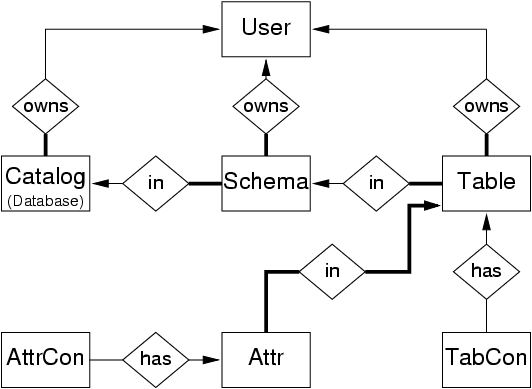
\psfig{file=Pic/catalog-er.ps}\end{center}

{\small (A small fragment of the meta-data tables in a typical RDBMS)}
\end{slide}

\begin{slide}
\ContHeading{Catalogs}
SQL:2003 standard view of metadata: @INFORMATION_SCHEMA@.

The @INFORMATION_SCHEMA@ is available globally and includes:

{\bf{Schemata}}(catalog\_name, schema\_name, schema\_owner, ...)

{\bf{Table}}(table\_catalog, table\_schema, table\_name, table\_type, ...)

{\bf{Column}}(table\_catalog, table\_schema, table\_name, column\_name, \\
~~~ ~~~ ~~~ ~~~ ordinal\_position, column\_default, data\_type, ...)

{\bf{View}}(table\_catalog, table\_schema, table\_name, view\_definition, ...)

{\bf{Table\_Constraint}}(..., constraint\_name, ..., constraint\_type, ...)

{\small etc. etc. etc.}
\end{slide}

\begin{slide}
\ContHeading{Catalogs}
DBMS internal meta-data is often different to standard, e.g.
\begin{indent}
\begin{small}
\begin{session}
    Users(id:int, name:string, ...)
    Databases(id:int, name:string, owner:ref(User), ...)
    Schemas(id:int, name:string, owner:ref(User), ...)
    Types(id:int, name:string, defn:string, size:int, ...)
    Tables(id:int, name:string, owner:ref(User),
                                    inSchema:ref(Schema), ...)
    Attributes(id:int, name:string, table:ref(Table),
                               type:ref(Type), pkey:bool, ...)
    TableConstraints(id:int, name:string, table:ref(Table),
                                             defn:string, ...)
    AttrConstraints(id:int, name:string, attr:ref(Attribute),
                                             defn:string, ...)
    {\textit{-- etc. etc. etc.}}
\end{session}
\end{small}
\end{indent}
\end{slide}

\begin{slide}
\ContHeading{Catalogs}
SQL DDL operations such as
\begin{indent}
\begin{small}
\begin{session}
    create table Abc (
        x integer primary key,
        y integer);
\end{session}
\end{small}
\end{indent}
are implemented internally as operations on meta-data, e.g.
\begin{indent}
\begin{small}
\begin{session}
    userID := current_user();
    schemaID := current_schema();
    tabID := nextval('tab_id_seq');
    select into intID id
    from Types where name='integer';
    insert into Tables(id,name,owner,inSchema,...)
           values (tabID, 'abc', userID, schema, ...)
    attrID := nextval('attr_id_seq');
    insert into Attributes(id,name,table,type,pkey,...)
           values (attrID, 'x', tabID, intID, true, ...)
    attrID := nextval('attr_id_seq');
    insert into Attributes(id,name,table,type,pkey,...)
           values (attrID, 'y', tabID, intID, false, ...)
\end{session}
\end{small}
\end{indent}
\end{slide}

\begin{slide}
\Heading{Access to System Catalog}
Users typically have access to the system catalog via
\begin{itemize}
\item special commands ~
	(e.g. PostgreSQL's @\d@, @\df@, etc.)
\item query-able views ~
	(e.g. Oracle's @select * from tab@)
\end{itemize}
How much is visible to each user depends on their role
\begin{itemize}
\item DBA can see/change anything in system catalog via SQL
\item ordinary user can see only some of the system catalog \\
	and can change it only via SQL DDL statements
\end{itemize}
\end{slide}

\begin{slide}
\Heading{PostgreSQL Catalog}
PostgreSQL stores catalog information as regular tables.

The @\d?@ special commands in @psql@ are just
wrappers around queries on those tables, e.g.


\begin{center}\begin{tabular}{lll}

\begin{minipage}{5cm}
@\dt@
 \\~\end{minipage}
 & \begin{minipage}{18cm}
list information about tables
\\~\end{minipage}
\\[1ex]

\begin{minipage}{5cm}
@\dv@
 \\~\end{minipage}
 & \begin{minipage}{18cm}
list information about views
\\~\end{minipage}
\\[1ex]

\begin{minipage}{5cm}
@\df@
 \\~\end{minipage}
 & \begin{minipage}{18cm}
list information about functions
\\~\end{minipage}
\\[1ex]

\begin{minipage}{5cm}
@\dp@
 \\~\end{minipage}
 & \begin{minipage}{18cm}
list table access privileges
\\~\end{minipage}
\\[1ex]

\begin{minipage}{5cm}
@\dT@
 \\~\end{minipage}
 & \begin{minipage}{18cm}
list information about data types
\\~\end{minipage}
\\[1ex]

\begin{minipage}{5cm}
@\dd@
 \\~\end{minipage}
 & \begin{minipage}{18cm}
shows comments attached to DB objects
\\~\end{minipage}
\\[1ex]
\end{tabular}
\end{center}

\end{slide}

\begin{slide}
\ContHeading{PostgreSQL Catalog}
A PostgreSQL installation typically has several databases.

Some catalog information is global, e.g.
\begin{itemize}
\item databases, users, ...
{\small 
\item there is one copy of each ``global'' table for the whole PostgreSQL installation
\vspace{-1ex}\item this copy is shared by all databases in the installation
}
\end{itemize}
Other catalog information is local to each database, e.g
\begin{itemize}
\item schemas, tables, attributes, functions, types, ...
{\small 
\item there is a separate copy of each ``local'' table in each database
\vspace{-1ex}\item a copy of each ``local'' table is made when a new database is created
}
\end{itemize}
\end{slide}

\begin{slide}
\ContHeading{PostgreSQL Catalog}
{\em{{\bf{@pg_shadow@}}}} contains information about database users:


\begin{center}\begin{tabular}{lll}

\begin{minipage}{5cm}@usename@ \\~\end{minipage}
 & \begin{minipage}{18cm}
symbolic user name (e.g. @jas@)
\\~\end{minipage}
\\[1ex]

\begin{minipage}{5cm}@usesysid@ \\~\end{minipage}
 & \begin{minipage}{18cm}
integer key to reference user
\\~\end{minipage}
\\[1ex]

\begin{minipage}{5cm}@passwd@ \\~\end{minipage}
 & \begin{minipage}{18cm}
md5-encrypted password
\\~\end{minipage}
\\[1ex]

\begin{minipage}{5cm}@usecreatdb@ \\~\end{minipage}
 & \begin{minipage}{18cm}
can create new databases
\\~\end{minipage}
\\[1ex]

\begin{minipage}{5cm}@usesuper@ \\~\end{minipage}
 & \begin{minipage}{18cm}
is a superuser (owns server process)
\\~\end{minipage}
\\[1ex]

\begin{minipage}{5cm}@usecatupd@ \\~\end{minipage}
 & \begin{minipage}{18cm}
can update system catalogs
\\~\end{minipage}
\\[1ex]
\end{tabular}
\end{center}

\end{slide}

\begin{slide}
\ContHeading{PostgreSQL Catalog}
{\em{{\bf{@pg_database@}}}} contains information about databases:


\begin{center}\begin{tabular}{lll}

\begin{minipage}{5cm}@datname@ \\~\end{minipage}
 & \begin{minipage}{18cm}
database name (e.g. @nssis@)
\\~\end{minipage}
\\[1ex]

\begin{minipage}{5cm}@datdba@ \\~\end{minipage}
 & \begin{minipage}{18cm}
database owner {\small (refs @pg_shadow.usesysid@)}
\\~\end{minipage}
\\[1ex]

\begin{minipage}{5cm}@datpath@ \\~\end{minipage}
 & \begin{minipage}{18cm}
where files for database are stored \\ {\small (if not in the PG\_DATA directory)}
\\~\end{minipage}
\\[1ex]

\begin{minipage}{5cm}@datacl@ \\~\end{minipage}
 & \begin{minipage}{18cm}
access permissions
\\~\end{minipage}
\\[1ex]
\end{tabular}
\end{center}

\end{slide}

\begin{slide}
\ContHeading{PostgreSQL Catalog}
{\em{{\bf{@pg_class@}}}} contains information about tables:


\begin{center}\begin{tabular}{lll}

\begin{minipage}{5cm}@relname@ \\~\end{minipage}
 & \begin{minipage}{18cm}
name of table (e.g. @employee@)
\\~\end{minipage}
\\[1ex]

\begin{minipage}{5cm}@relnamespace@ \\~\end{minipage}
 & \begin{minipage}{18cm}
schema in which table defined \\
{\small (refs @pg_namespace.oid@)}
\\~\end{minipage}
\\[1ex]

\begin{minipage}{5cm}@reltype@ \\~\end{minipage}
 & \begin{minipage}{18cm}
data type corresponding to table \\
{\small (refs @pg_type.oid@)}
\\~\end{minipage}
\\[1ex]

\begin{minipage}{5cm}@relowner@ \\~\end{minipage}
 & \begin{minipage}{18cm}
owner {\small (refs @pg_shadow.usesysid@)}
\\~\end{minipage}
\\[1ex]

\begin{minipage}{5cm}@reltuples@ \\~\end{minipage}
 & \begin{minipage}{18cm}
\# tuples in table
\\~\end{minipage}
\\[1ex]

\begin{minipage}{5cm}@relacl@ \\~\end{minipage}
 & \begin{minipage}{18cm}
access permissions
\\~\end{minipage}
\\[1ex]
\end{tabular}
\end{center}

{\small 
Also holds info about objects other than tables, e.g. views, sequences, indexes.
}
\end{slide}

\begin{slide}
\ContHeading{PostgreSQL Catalog}
{\em{{\bf{@pg_class@}}}} also holds various flags/counters for each
table:


\begin{center}\begin{tabular}{lll}

\begin{minipage}{5cm}@relkind@ \\~\end{minipage}
 & \begin{minipage}{18cm}
what kind of object \\
{\small 
'r' = ordinary table, 'i' = index, 'v' = view \\
'c' = composite type, 'S' = sequence, 's' = special
}
\\~\end{minipage}
\\[1ex]

\begin{minipage}{5cm}@relnatts@ \\~\end{minipage}
 & \begin{minipage}{18cm}
\# attributes in table \\
{\small (how many entries in @pg_attribute@ table)}
\\~\end{minipage}
\\[1ex]

\begin{minipage}{5cm}@relchecks@ \\~\end{minipage}
 & \begin{minipage}{18cm}
\# of constraints on table \\
{\small (how many entries in @pg_constraint@ table)}
\\~\end{minipage}
\\[1ex]

\begin{minipage}{5cm}@relhasindex@ \\~\end{minipage}
 & \begin{minipage}{18cm}
table has/had an index?
\\~\end{minipage}
\\[1ex]

\begin{minipage}{5cm}@relhaspkey@ \\~\end{minipage}
 & \begin{minipage}{18cm}
table has/had a primary key?
\\~\end{minipage}
\\[1ex]
\end{tabular}
\end{center}

etc.
\end{slide}

\begin{slide}
\ContHeading{PostgreSQL Catalog}
{\em{{\bf{@pg_type@}}}} contains information about data types:


\begin{center}\begin{tabular}{lll}

\begin{minipage}{5cm}@typname@ \\~\end{minipage}
 & \begin{minipage}{18cm}
name of type (e.g. @integer@)
\\~\end{minipage}
\\[1ex]

\begin{minipage}{5cm}@typnamespace@ \\~\end{minipage}
 & \begin{minipage}{18cm}
schema in which type defined \\
{\small (refs @pg_namespace.oid@)}
\\~\end{minipage}
\\[1ex]

\begin{minipage}{5cm}@typowner@ \\~\end{minipage}
 & \begin{minipage}{18cm}
owner {\small (refs @pg_shadow.usesysid@)}
\\~\end{minipage}
\\[1ex]

\begin{minipage}{5cm}@typtype@ \\~\end{minipage}
 & \begin{minipage}{18cm}
what kind of data type \\
{\small  'b' = base type, 'c' = complex (row) type, ... }
\\~\end{minipage}
\\[1ex]

\begin{minipage}{5cm}@typlen@ \\~\end{minipage}
 & \begin{minipage}{18cm}
how much storage used for type values \\
{\small (-1 for variable-length types, e.g. @text@)}
\\~\end{minipage}
\\[1ex]

\begin{minipage}{5cm}@typrelid@ \\~\end{minipage}
 & \begin{minipage}{18cm}
table associated to complex type \\
{\small (refs @pg_class.oid@)}
\\~\end{minipage}
\\[1ex]
\end{tabular}
\end{center}

etc.
\end{slide}

\begin{slide}
\ContHeading{PostgreSQL Catalog}
{\em{{\bf{@pg_attribute@}}}} contains information about attributes:


\begin{center}\begin{tabular}{lll}

\begin{minipage}{5cm}@attname@ \\~\end{minipage}
 & \begin{minipage}{18cm}
name of attribute (e.g. @id@)
\\~\end{minipage}
\\[1ex]

\begin{minipage}{5cm}@attrelid@ \\~\end{minipage}
 & \begin{minipage}{18cm}
table this attribute belongs to \\
{\small (refs @pg_class.oid@)}
\\~\end{minipage}
\\[1ex]

\begin{minipage}{5cm}@atttypid@ \\~\end{minipage}
 & \begin{minipage}{18cm}
data type of this attribute \\
{\small (refs @pg_type.oid@)}
\\~\end{minipage}
\\[1ex]

\begin{minipage}{5cm}@attlen@ \\~\end{minipage}
 & \begin{minipage}{18cm}
storage space required by attribute \\
{\small (a copy of @pg_type.typlen@ for data type)}
\\~\end{minipage}
\\[1ex]

\begin{minipage}{5cm}@attnum@ \\~\end{minipage}
 & \begin{minipage}{18cm}
attribute position {\small (1..n, sys attrs are -ve)}
\\~\end{minipage}
\\[1ex]
\end{tabular}
\end{center}

\end{slide}

\begin{slide}
\ContHeading{PostgreSQL Catalog}
{\em{{\bf{@pg_attribute@}}}} also holds constraint/status information:


\begin{center}\begin{tabular}{lll}

\begin{minipage}{5cm}@attnotnull@ \\~\end{minipage}
 & \begin{minipage}{18cm}
attribute may not be null?
\\~\end{minipage}
\\[1ex]

\begin{minipage}{5cm}@atthasdef@ \\~\end{minipage}
 & \begin{minipage}{18cm}
attribute has a default values \\
{\small (value is held in @pg_attrdef@ table)}
\\~\end{minipage}
\\[1ex]

\begin{minipage}{5cm}@attisdropped@ \\~\end{minipage}
 & \begin{minipage}{18cm}
attribute has been dropped from table
\\~\end{minipage}
\\[1ex]
\end{tabular}
\end{center}

plus others related to strage properties of attribute.
\end{slide}

\begin{slide}
\ContHeading{PostgreSQL Catalog}
{\em{{\bf{@pg_proc@}}}} contains information about functions:


\begin{center}\begin{tabular}{lll}

\begin{minipage}{5cm}@proname@ \\~\end{minipage}
 & \begin{minipage}{18cm}
name of function (e.g. @substr@)
\\~\end{minipage}
\\[1ex]

\begin{minipage}{5cm}@pronamespace@ \\~\end{minipage}
 & \begin{minipage}{18cm}
schema in which function defined \\
{\small (refs @pg_namespace.oid@)}
\\~\end{minipage}
\\[1ex]

\begin{minipage}{5cm}@proowner@ \\~\end{minipage}
 & \begin{minipage}{18cm}
owner {\small (refs @pg_shadow.usesysid@)}
\\~\end{minipage}
\\[1ex]

\begin{minipage}{5cm}@prolang@ \\~\end{minipage}
 & \begin{minipage}{18cm}
what language function written in
\\~\end{minipage}
\\[1ex]

\begin{minipage}{5cm}@proacl@ \\~\end{minipage}
 & \begin{minipage}{18cm}
access control
\\~\end{minipage}
\\[1ex]
\end{tabular}
\end{center}

etc.
\end{slide}

\begin{slide}
\ContHeading{PostgreSQL Catalog}
{\em{{\bf{@pg_proc@}}}} contains information about arguments:


\begin{center}\begin{tabular}{lll}

\begin{minipage}{5cm}@pronargs@ \\~\end{minipage}
 & \begin{minipage}{18cm}
how many arguments
\\~\end{minipage}
\\[1ex]

\begin{minipage}{5cm}@prorettype@ \\~\end{minipage}
 & \begin{minipage}{18cm}
return type {\small (refs @pg_type.oid@)}
\\~\end{minipage}
\\[1ex]

\begin{minipage}{5cm}@proargtypes@ \\~\end{minipage}
 & \begin{minipage}{18cm}
argument types {\small (vector of refs @pg_type.oid@)}
\\~\end{minipage}
\\[1ex]

\begin{minipage}{5cm}@proisstrict@ \\~\end{minipage}
 & \begin{minipage}{18cm}
returns null if any arg is null
\\~\end{minipage}
\\[1ex]

\begin{minipage}{5cm}@prosrc@ \\~\end{minipage}
 & \begin{minipage}{18cm}
source code if interpreted {\small (e.g. PLpgSQL)}
\\~\end{minipage}
\\[1ex]
\end{tabular}
\end{center}

\end{slide}

\begin{slide}
\ContHeading{PostgreSQL Catalog}
{\em{{\bf{@pg_constraints@}}}} contains information about constraints:


\begin{center}\begin{tabular}{lll}

\begin{minipage}{5cm}@conname@ \\~\end{minipage}
 & \begin{minipage}{18cm}
name of constraint {\small (not unique)}
\\~\end{minipage}
\\[1ex]

\begin{minipage}{5cm}@connamespace@ \\~\end{minipage}
 & \begin{minipage}{18cm}
schema containing this constraint
\\~\end{minipage}
\\[1ex]

\begin{minipage}{5cm}@contype@ \\~\end{minipage}
 & \begin{minipage}{18cm}
kind of constraint \\
{\small 
'c' = check, 'u' = unique, \\
'p' = primary key, 'f' = foreign key
}
\\~\end{minipage}
\\[1ex]

\begin{minipage}{5cm}@conrelid@ \\~\end{minipage}
 & \begin{minipage}{18cm}
which table {\small (refs @pg_class.oid@)}
\\~\end{minipage}
\\[1ex]

\begin{minipage}{5cm}@conkey@ \\~\end{minipage}
 & \begin{minipage}{18cm}
which attributes \\
{\small (vector of values from @pg_attribute.attnum@)}
\\~\end{minipage}
\\[1ex]

\begin{minipage}{5cm}@consrc@ \\~\end{minipage}
 & \begin{minipage}{18cm}
check constraint expression
\\~\end{minipage}
\\[1ex]
\end{tabular}
\end{center}

\end{slide}

\begin{slide}
\ContHeading{PostgreSQL Catalog}
For full details on PostgreSQL catalogs:

{\em{PostgreSQL 8.0.1 Developer's Guide}}

Part VII, Chapter 41, System Catalogs

Part IV, Chapter 30, The Information Schema
\end{slide}

\begin{slide}
\Heading{Security, Privilege, Authorisation}
\end{slide}

\begin{slide}
\Heading{Database Security}
Database security has to meet the following objectives:
\begin{itemize}
\item
{\em{Secrecy}}:
	information not disclosed to unauthorised users \\
	{\small e.g. a student should {\bf{not}} be able to examine other students' marks}
\item
{\em{Integrity}}:
 	only authorised users are allowed to modify data \\
	{\small e.g. a student should not be able to modify anybody's marks}
\item
{\em{Availability}}:
	authorised users should not be denied access \\
	{\small e.g. the LIC should be able to read/changes marks for their course}
\end{itemize}
{\small 
Goal: prevent unauthorised use/alteration/destruction of mission-critical data.
}
\end{slide}

\begin{slide}
\ContHeading{Database Security}
Security mechanisms operate at a number of levels
\begin{itemize}
\item within the database system ~ (SQL-level privileges) \\
	{\small e.g. specific users can query/modify/update only specified database objects}
\item accessing the database system ~ (users/passwords) \\
	{\small e.g. users are required to authenticate themselves at connection-time}
\item operating system ~ (access to DB clients) \\
	{\small e.g. users should not obtain access to the DBMS superuser account}
\item network ~ (most DB access nowadays is via network) \\
	{\small e.g. results should not be transmitted unencrypted to Web browsers}
\item human/physical ~ (conventional security mechanisms) \\
	{\small e.g. no unauthorised physical access to server hosting the DBMS}
\end{itemize}
\end{slide}

\begin{slide}
\Heading{Database Access Control}
Access to DBMSs involves two aspects:
\begin{itemize}
\item having execute permission for a DBMS client {\small (e.g. @psql@)}
\item having a username/password registered in the DBMS
\end{itemize}
Establishing a {\em{connection}} to the database:
\begin{itemize}
\item user supplies {\em{database}}/{\em{username}}/{\em{password}} to client
\item client passes these to server, which validates them
\item if valid, user is ``logged in'' to the specified database
\end{itemize}
\end{slide}

\begin{slide}
\ContHeading{Database Access Control}
Note: we don't need to supply username/password to @psql@
\begin{itemize}
\item @psql@ works out which user by who ran the client process
\item we're all PostgreSQL super-users on our own servers
\item servers are configured to allow super-user direct access
\end{itemize}

Note: access to databases via the Web involves:
\begin{itemize}
\item running a script on a Web server
\item using the Web server's access rights on the DBMS
\end{itemize}
\end{slide}

\begin{slide}
\ContHeading{Database Access Control}
Database {\em{users}} are set up by the DBA via the command:
\begin{syntax}
    CREATE USER \(Name\) IDENTIFIED BY '\(Password\)'
\end{syntax}
Various privileges can be assigned at user-creation time, e.g.
\begin{itemize}
\item ability to create new users or databases or tables
\end{itemize}
User properties may be subsequently changed via:
\begin{syntax}
    ALTER USER \(Name\) IDENTIFIED BY '\(NewPassword\)'
\end{syntax}
This command is also used to change privileges, quotas, etc.
\end{slide}

\begin{slide}
\ContHeading{Database Access Control}
A user may be associated with a {\em{role}} or {\em{group}}
\begin{itemize}
\item which typically gives them additional specific privileges
\end{itemize}
Roles are also set up by the DBA via the command:
\begin{syntax}
    CREATE ROLE \(RoleName\)
\end{syntax}
Examples of roles:
\begin{itemize}
\item AcademicStaff ... has privileges to read/modify marks
\item OfficeStaff ... has privilege to read all marks
\item Student ... has privilege to read own marks only
\end{itemize}
\end{slide}

\begin{slide}
\Heading{Database Access Control in PostgreSQL}
PostgreSQL has two ways to create users ...

From the Unix command line, via the command
\begin{syntax}
    createuser [ -a | -d ] \(Name\) 
\end{syntax}
{\small 
(@-a@ allows user to create other users, ~ @-d@ allows user to create databases)
}

From SQL, via the statement:
\begin{syntax}
    CREATE USER \(UserName\) \(Options\)
    {\textit{-- where \(Options\) are any of ...}}
    WITH PASSWORD '\(Password\)'
    CREATEDB | NOCREATEDB
    CREATEUSER | NOCREATEUSER
    IN GROUP \(GroupName\)
    VALID UNTIL '\(TimeStamp\)'
\end{syntax}
\end{slide}

\begin{slide}
\ContHeading{Database Access Control in PostgreSQL}
PostgreSQL uses {\em{group}} rather than {\em{role}}
	~ {\small (diff terminology only)}.

Groups are created via the SQL statement
\begin{syntax}
    CREATE GROUP \(GroupName\)
    WITH USER \(UserName1\), \(UserName2\), ...
\end{syntax}
and may be subsequently modified by
\begin{syntax}
    ALTER GROUP \(GroupName\)
    ADD USER \(UserName1\), \(UserName2\), ...
    {\textit{--and}}
    ALTER GROUP \(GroupName\)
    DROP USER \(UserName1\), \(UserName2\), ...
\end{syntax}
\end{slide}

\begin{slide}
\ContHeading{Database Access Control in PostgreSQL}
PostgreSQL stores user information in a table @pg_shadow@.

Each user is associated with a unique identifying number.

Every PostgreSQL is created with a default user (id=1, superuser).

Some fields in the @pg_shadow@ table:
\begin{itemize}
\vspace{-1ex}\item @usename@: string for user name (e.g. @jas@)
\vspace{-1ex}\item @usesysid@: unqiue user id (e.g. 1, 100, ...)
\vspace{-1ex}\item @usecreatedb@: can user create new databases?
\vspace{-1ex}\item @usesuper@: is the user a superuser?
\vspace{-1ex}\item @usecatupd@: can user update system catalogues?
\vspace{-1ex}\item @passwd@: encrypted version of user's password
\end{itemize}
\end{slide}

\begin{slide}
\ContHeading{Database Access Control in PostgreSQL}
PostgreSQL uses a file called @pg_hba.conf@ to determine
how to authenticate users
{\small (@hba@ stands for host-based authentication)}.

This file contains a sequence of entries where each entry has:
\begin{itemize}
\item connection method {\small (Unix-domain socket, TCP/IP, encrypted)}
\item list of databases (or @all@)
\item user/group name (or @all@)
\item IP address and IP mask
\item authentication method (plus options)
\end{itemize}
PostgreSQL uses first four items to determine authentication method.
\end{slide}

\begin{slide}
\ContHeading{Database Access Control in PostgreSQL}
Possible authentication methods:
\begin{itemize}
\item @md5@: get password from user, check against @pg_shadow@
\item @krb5@: use Kerberos-based authentication
\item @reject@: do not allow the user to access DBMS this way
\item @trust@: allow them to log in as any user without password
\item @ident@: allow them access based on Unix user name info
\begin{itemize}
\item @ident@+map: see if UnixName is member of map list
\item @ident@+@sameuser@: log in as user with name UnixName
\end{itemize}
\end{itemize}
\end{slide}

\begin{slide}
\ContHeading{Database Access Control in PostgreSQL}
Examples from @pg_hba.conf@ file:
\begin{indent}
\begin{small}
\begin{session}
    # Allow any user on the local system to connect to any database
    # as any user if accessing from local machine via Unix socket.
    #
    #{\em{TYPE  DATABASE USER IP-ADDRESS    IP-MASK          METHOD}}
    {\bf{{\em{local  all      all                                 trust}}}}
    
    # Reject all connection from 192.168.54.1
    # 
    #{\em{TYPE  DATABASE  USER IP-ADDRESS    IP-MASK          METHOD}}
    {\bf{{\em{host   all       all  192.168.54.1  255.255.255.255  reject}}}}
    
    # Allow any user from any host with IP address 192.168.93.x
    # to connect to database "mydb" as the same user name that
    # ident reports for the connection (typically Unix user name).
    # 
    #{\em{TYPE  DATABASE USER IP-ADDRESS    IP-MASK        METHOD}}
    {\bf{{\em{host   mydb     all  192.168.93.0  255.255.255.0  ident sameuser}}}}
    
    # Allow a user from host 192.168.12.10 to connect to database
    # "mydb" only if the user's password is correctly supplied.
    # 
    #{\em{TYPE  DATABASE USER IP-ADDRESS    IP-MASK          METHOD}}
    {\bf{{\em{host   mydb     all  192.168.12.10 255.255.255.255  md5}}}}
\end{session}
\end{small}
\end{indent}
\end{slide}

\begin{slide}
\Heading{SQL Access Control}
SQL access control deals with
\begin{itemize}
\item privileges on database objects
	{\small (e.g. tables, view, functions, ...)}
\item allocating such privileges to users and/or roles
\end{itemize}
The user who creates an object is automatically assigned:
\begin{itemize}
\item ownership of that object
\item a privilege to modify (@ALTER@) the object
\item a privilege to remove (@DROP@) the object
\item along with all other privileges specified below
\end{itemize}
\end{slide}

\begin{slide}
\ContHeading{SQL Access Control}
The owner of an object can assign privileges on that object
to other users.

Accomplished via the command:
\begin{syntax}
    GRANT \(Privileges\) ON \(Object\)
    TO \(list of\) (\(Users\)|\(Roles\)) | PUBLIC
    [ WITH GRANT OPTION ]
\end{syntax}

$Privileges$ can be @ALL@
	{\small (giving everything but @ALTER@ and @DROP@)}

@WITH GRANT OPTION@ allows a user who has been granted a privilege
to pass the privilege on to any other user.
\end{slide}

\begin{slide}
\ContHeading{SQL Access Control}
Effects of privilege granting
\begin{itemize}
\item are sometimes subtle (possible conflicts?)
\item can be represented by an {\em{authorisation graph}}
\end{itemize}
\vspace*{1cm}\begin{center}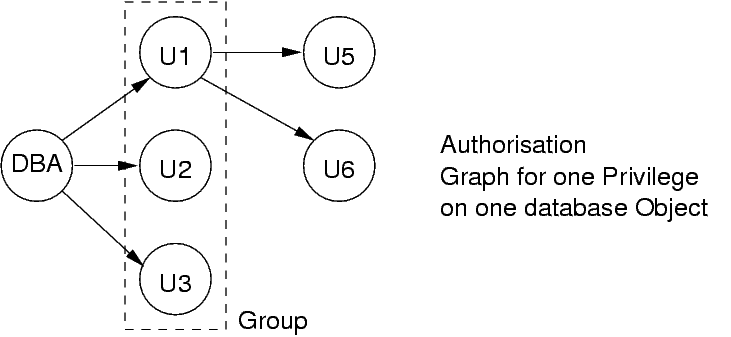
\psfig{file=Pic/auth-graph.ps}\end{center}
\end{slide}

\begin{slide}
\ContHeading{SQL Access Control}
Privileges can be withdrawn via the command:
\begin{syntax}
    REVOKE \(Privileges\) ON \(Object\)
    FROM \(ListOf\) (\(Users\)|\(Roles\)) | PUBLIC
    CASCADE | RESTRICT
\end{syntax}
Normally withdraws Privileges from just specified users/roles.

@CASCADE@ ... also withdraws from users they had granted to.

E.g. revoking from U1 also revokes U5 and U6

@RESTRICT@ ... fails if users had granted privileges to others.

E.g. revoking from U1 fails, revoking U5 or U2 succeeds
\end{slide}

\begin{slide}
\ContHeading{SQL Access Control}
Privileges available for users on database objects:

@SELECT@:
\begin{itemize}
\item user can read all rows and columns of table/view
\item this includes columns added later via @ALTER TABLE@
\end{itemize}
@INSERT@ ~ or ~ @INSERT(@$ColName$@)@:
\begin{itemize}
\item user can insert rows into table
\item if $ColName$ specified, can only set value of that column
\end{itemize}
\end{slide}

\begin{slide}
\ContHeading{SQL Access Control}
More privileges available for users on database objects:

@UPDATE@ ~ or ~ @UPDATE(@$ColName$@)@:
\begin{itemize}
\item user can modify values stored in the table
\item if $ColName$ specified, can only set value of that column
\end{itemize}
@DELETE@:
\begin{itemize}
\item user can delete rows from the table
\item this does {\it{not}} imply permission to remove table itself \\
	{\small (this is the @DROP@ privilege automatically assigned to the object creator)}
\end{itemize}
\end{slide}

\begin{slide}
\ContHeading{SQL Access Control}
More privileges available for users on database objects:

@REFERENCES(@$ColName$@)@:
\begin{itemize}
\item user can use $ColName$ as foreign key in their tables
\end{itemize}
@EXECUTE@:
\begin{itemize}
\item user can execute the specified function
\end{itemize}
@TRIGGER@:
\begin{itemize}
\item user is allowed to create triggers on a table
\item note that tiggers always execute with creator's privileges
\end{itemize}
\end{slide}

\begin{slide}
\Heading{SQL Access Control in PostgreSQL}
PostgreSQL follows the above with some minor variations:
\begin{itemize}
\item group names must be preceded by @GROUP@
\item there is an additional privilege for @RULE@s
\end{itemize}
See the PostgreSQL manual for full details.
\end{slide}

\begin{slide}
\Heading{Problems with SQL Access Control}
Allowing users to assign privileges to others can be exploited.

Example: student S wants access to table of marks M 
\begin{itemize}
\item M is owned by lecturer L, S has no SELECT privilege on M
\item S creates a new table SS and grants INSERT privilege to L
\item S modifies code of some PLpgSQL function F used by L
\item the modifications to F copy the data from M into SS
\item S restores F to its original state
	{\small (in case L gets suspicious)}
\item S now has access to the data from M in table SS
\end{itemize}
\end{slide}

\begin{slide}
\Heading{Mandatory Access Control}
Above approach is called {\em{discretionary access control}}
\begin{itemize}
\item relies on individual users to assign privileges
\item very fine-grained $\Rightarrow$ tedious to specify privileges
\end{itemize}
An alternative approach: {\em{manadatory access control}} {\small (MAC)}
\begin{itemize}
\item global approach to access control; simple to specify
\item currently under development ~ {\small (not yet available in DBMSs)}
\item a popular MAC model is Bell-LaPadula
	~ {\small (see next page)}
\end{itemize}
\end{slide}

\begin{slide}
\ContHeading{Mandatory Access Control}
Access control is described in terms of ...
\begin{itemize}
\item {\em{objects}}
	{\small (e.g. tables, rows, views, columns, ...)}
\item {\em{subjects}}
	{\small (e.g. users, programs, ...)}
\item {\em{security classes}}
	{\small (an ordered collection, least to most secure)}
\end{itemize}
Example: $Unclassified < Confidential < Secret < Top Secret$

Subjects and objects are assigned to security classes.

Impose these restrictions on every data access:
\begin{itemize}
\item subject S can read object O only if class(S) $\geq$ class(O)
\item subject S can write object O only if class(S) $\leq$ class(O)
\end{itemize}
\end{slide}

\begin{slide}
\Heading{Security in Statistical Databases}
{\em{Statistical databases}}
\begin{itemize}
\item contain data about a group of individuals
\item but allow access only to summary data
\item also provide controls to select subsets of data
\end{itemize}
Example of such a database: population census
\begin{itemize}
\vspace{-1ex}\item information is stored about individuals
\vspace{-1ex}\item users are only allowed to examine trends/summaries
\vspace{-1ex}\item e.g. can find out average age of people living in Sydney \\
but cannot ask the question ``How old is John?''
\end{itemize}
Privacy is protected, but useful information is still available.
\end{slide}

\begin{slide}
\ContHeading{Security in Statistical Databases}
Consider: anonymous surveys in an on-line survey system
\begin{itemize}
\item can see overall results ~ {\small (e.g. tutorials rated at 7/10)}
\item but do not have access to individual student responses
\item can also summarize results for subgroups \\
	{\small (e.g. CE students rated tutorials at 6/10, CS students rated tutorials at 8/10)}
\end{itemize}
Problem: subset controls may allow selection of individuals, e.g.
\begin{itemize}
\item we know that there's only one Law student in the class
\item ask for a ``summary'' of responses given by Law students
\end{itemize}
\end{slide}

\begin{slide}
\ContHeading{Security in Statistical Databases}
How to solve this problem?
\begin{itemize}
\item restrict subsets to being larger than a minimum size $N$
\end{itemize}
But still doesn't quite work, e.g.
\begin{itemize}
\item system gives summaries for several groups (e.g. SE+CE)
\item get summary for Law+CE ~ {\small (presumably with $>N$ responses)}
\item get summary just for CE ~ {\small (assume count of reponses given)}
\item determine Law response from the ``difference''
\end{itemize}
{\small 
Security is difficult to enforce in statistical databases, but activity can be logged.
}
\end{slide}

\begin{slide}
\Heading{Performance Tuning}
\end{slide}

\begin{slide}
\Heading{Performance Tuning}
Schema design:
\begin{itemize}
\item devise data structures to {\em{represent application information}}
\end{itemize}
Performance tuning:
\begin{itemize}
\item devise data structures to {\em{achieve good performance}}
\end{itemize}
Good performance may involve any/all of:
\begin{itemize}
\vspace{-1ex}\item making applications run faster
\vspace{-1ex}\item lowering response time of queries/transactions
\vspace{-1ex}\item improving overall transaction throughput
\end{itemize}
\end{slide}

\begin{slide}
\ContHeading{Performance Tuning}
Tuning requires us to consider the following:
\begin{itemize}
\item which queries and transactions will be used? \\
	~ {\small (e.g. check balance for payment, display recent transaction history)}
\item how frequently does each query/transaction occur? \\
	~ {\small (e.g. 99\% of transactions are EFTPOS payments; 1\% are print balance)}
\item are there time constraints on queries/transactions? \\
	~ {\small (e.g. payment at EFTPOS terminals must be approved within 7 seconds)}
\item are there uniqueness constraints on any attributes? \\
	~ {\small (therefore, define index on attributes to speed up insertion uniqueness check)}
\item how frequently do updates occur? \\
	~ {\small (indexes slow down updates, because must update table {\it{and}} index)}
\end{itemize}
\end{slide}

\begin{slide}
\ContHeading{Performance Tuning}
Performance can be considered at two times:
\begin{itemize}
\item {\it{during}} schema design
\begin{itemize}
\item typically towards the end of schema design process
\item requires schema transformations such as denormalisation
\end{itemize}
\item {\it{after}} schema design
\begin{itemize}
\item requires adding extra data structures such as indexes
\end{itemize}
\end{itemize}
\end{slide}

\begin{slide}
\Heading{Denormalisation}
Normalisation structures data to minimise storage redundancy.
\begin{itemize}
\vspace{-1ex}\item achieves this by ``breaking up'' the data into logical chunks
\vspace{-1ex}\item requires minimal ``maintenance'' to ensure data consistency
\end{itemize}
Problem: queries that need to put data back together.
\begin{itemize}
\vspace{-1ex}\item need to use a (potentially expensive) join operation
\vspace{-1ex}\item if an expensive join is frequent, system performance suffers
\end{itemize}
Solution: store some data redundantly
\begin{itemize}
\vspace{-1ex}\item benefit: queries needing expensive join are now cheap
\vspace{-1ex}\item trade-off: extra maintenance effort to maintain consistency
\vspace{-1ex}\item worthwhile if joins are frequent and updates are rare
\end{itemize}
\end{slide}

\begin{slide}
\ContHeading{Denormalisation}
Example: Courses = Course $\bowtie$ Subject $\bowtie$ Term

If we frequently need to refer to course ``standard'' name
\begin{itemize}
\item add extra @courseName@ column into @Course@ table
\item cost: trigger before insert on @Course@ to construct name
\item trade-off likely to be worthwhile: @Course@ insertions infrequent
\end{itemize}
\begin{indent}
\begin{small}
\begin{session}
    {\textit{-- can now replace a query like:}}
    select s.code||t.year||t.sess, e.grade, e.mark
    from   Course c, CourseEnrolment e, Subject s, Term t
    where  e.course = c.id and c.subject = s.id and c.term = t.id
    {\textit{-- by a query like:}}
    select c.courseName, e.grade, e.mark
    from   Course c, CourseEnrolment e
    where  e.course = c.id 
\end{session}
\end{small}
\end{indent}
\end{slide}

\begin{slide}
\Heading{Indexes}
Indexes provide efficient content-based access to tuples.

Can build indexes on any (combination of) attributes.

Definining indexes:
\begin{syntax}
    CREATE INDEX \(name\) ON \(table\) ( \(attr\sb{1}\), \(attr\sb{2}\), ... )
\end{syntax}
$attr_{i}$ can be an arbitrary expression (e.g. @upper(name)@).

@CREATE INDEX@ also allows us to specify
\begin{itemize}
\vspace{-1ex}\item that the index is on @UNIQUE@ values
\vspace{-1ex}\item an access method (@USING@ btree, hash, rtree, or gist)
\end{itemize}
\end{slide}

\begin{slide}
\ContHeading{Indexes}
Indexes can make a huge difference to query processing cost.

On the other hand, they introduce overheads (storage, updates).

Creating indexes to maximise performance benefits:
\begin{itemize}
\item apply to attributes used in equality/range conditions, e.g.
\begin{indent}
\begin{small}
\begin{session}
    select * from Employee where {\em{id}} = 12345
    select * from Employee where {\em{age}} > 60
    select * from Employee where {\em{salary}} between 10000 and 20000
\end{session}
\end{small}
\end{indent}
\item but only in queries that are frequently used
\item and on tables that are not updated frequently
\end{itemize}
\end{slide}

\begin{slide}
\ContHeading{Indexes}
Considerations in applying indexes:
\begin{itemize}
\item is an attribute used in frequent/expensive queries? \\
	~ {\small (note that some kinds of queries can be answered from index alone)}
\item should we create an index on a collection of attributes? \\
	~ {\small (yes, if the collection is used in a frequent/expensive query)}
\item can we exploit a clustered index? {\small (only one per table)}
\item should we use B-tree or Hash index?
\begin{indent}
\begin{small}
\begin{session}
    {\textit{-- use hashing for (unique) attributes in equality tests, e.g.}}
    select * from Employee where {\em{id}} = 12345
    {\textit{-- use B-tree for attributes in range tests, e.g.}}
    select * from Employee where {\em{age}} > 60
\end{session}
\end{small}
\end{indent}
\end{itemize}
\end{slide}

\begin{slide}
\Heading{Query Tuning}
Sometimes, a query can be re-phrased to affect performance:
\begin{itemize}
\item by helping the optimiser to make use of indexes
\item by avoiding (unnecessary) operations that are expensive
\end{itemize}
Examples which {\it{may}} prevent optimiser from using indexes:
\begin{indent}
\begin{session}
    select name from Employee where {\em{salary}}/365 > 10.0
           {\textit{-- fix by re-phrasing condition to (salary > 3650)}}
    select name from Employee where {\em{name}} like '\%ith\%'
    select name from Employee where {\em{birthday}} is null
           {\textit{-- above two are difficult to "fix"}}
    select name from Employee
    where  dept in (select id from Dept where ...)
           {\textit{-- fix by using Employee join Dept on (e.dept=d.id)}}
\end{session}
\end{indent}
\end{slide}

\begin{slide}
\ContHeading{Query Tuning}
Other factors to consider in query tuning:
\begin{itemize}
\item @select distinct@ requires a sort; is @distinct@ necessary?
\item if multiple join conditions are available ... \\
	choose join attributes that are indexed, avoid joins on strings
\begin{indent}
\begin{small}
\begin{session}
    select ... Employee join Customer on (s.{\em{name}} = p.{\em{name}})
    {\textit{vs}}
    select ... Employee join Customer on (s.{\em{ssn}} = p.{\em{ssn}})
\end{session}
\end{small}
\end{indent}
\item sometimes @or@ in condition prevents index from being used ... \\
	replace the @or@ condition by a union of non-@or@ clauses
\begin{indent}
\begin{small}
\begin{session}
    select name from Employee where dept=1 or dept=2
    {\textit{vs}}
    (select name from Employee where {\em{dept}}=1)
    union
    (select name from Employee where {\em{dept}}=2)
\end{session}
\end{small}
\end{indent}
\end{itemize}
\end{slide}

\end{lecture}
